%
% Test exam document for Course INLMIC (Inleiding Microcontrollers)
% at The Hague University of Applied Sciences, Electrical Engineering.
%
% (c)2014, J. op den Brouw <J.E.J.opdenBrouw@hhs.nl>
% v0.5 - 24 sept 2013
% v0.6 - 13 nov 2013: added automatic answer rendering and file output
% v0.7 -  2 sep 2014: changed to tisdexam document class
%                     redef \qformat
% v0.8 - 22 oct 2014: changed lots of solutions
% v.081- 29 oct 2014: changed PD2, PD2 to PD3, PD2 (Ruben Ijlst)
% v0.9 - 27 aug 2018: changed all verbatim to listings. 
%
% This tex document makes use of the exam class.
%


%% 12pt charachters, A4 paper size, one side printing, equation left aligned
\documentclass[a4paper,12pt,fleqn,dutch,mimicwordtwentyten]{tisdexam}
%\documentclass[a4paper,12pt,fleqn,dutch,mimicwordtwentyten,answers]{tisdexam}
%                                                           ^^^^^^^
%                                           remove answers for no answers/solutions

% User adjustable commands
\opleiding{Elektrotechniek}
\opsteller{J.E.J. op den Brouw}
\tweedelezer{B. Kuiper}
\toetsnaam{INLMIC (proeftoets)}
\toetsnaamkort{INLMIC (proeftoets)}
\groep{EQ1, EQ3D}
\toetsdatum{1 januari 1970}
\toetsdatumkort{01-01-1970}
\tijd{0:00 -- 1:30}
\aantalbladzijden{\numpages}
\aantalvragen{\numquestions}
\opmerkingen{Aantekeningen, boeken, afdrukken van de PowerPoint-slides}
\cesuur{Beoordeling tentamen: Elk goed antwoord levert 90/\numquestions{} punten op, in totaal zijn 90 punten te behalen. \newline Eindcijfer = 1 + (aantal behaalde punten / 10)}
\module{}

\gelinieerdpapiertrue
\kladpapiertrue
\antwoordformulierabcdetrue

\eenvoudigerekenmachinetrue
\tekenbenodigdhedentrue
\grafischerekenmachinetrue
\eigenaantekeningentrue
\boekendictatentrue

\eigenaantekeningen{zie Opmerkingen}
\boekendictaten{zie Opmerkingen}

\documentengesorteerddocumenttrue

%% Set input encoding to ISO-8859-1 (latin1)
\usepackage[latin1]{inputenc}
\usepackage[T1]{fontenc}

%% Use packages...
\usepackage{array}
\setlength{\mathindent}{1em}

%% PDF Version and compression...
\pdfminorversion=5
\pdfobjcompresslevel=2

%% Include graphics files
\usepackage{graphicx}

%% Enumerate items
\usepackage{enumitem}

%% Using floats
\usepackage{float}

%% Use the AMS Mathematical characters
\usepackage{mathtools}
%%%\usepackage{amsfonts}
%%%\usepackage{amssymb}


\ifx \dyslect \undefined
	%% Use Times
	\usepackage{mathptmx}
\else
	%% Use Helvetica instead of Times
	\usepackage[scaled]{helvet}
	\renewcommand*\familydefault{\sfdefault} %% Only if the base font of the document is to be sans serif
\fi

%% Making captions nicer...
\usepackage[font=footnotesize,format=plain,labelfont={bf,up},textfont={it,up}]{caption}
\captionsetup[table]{justification=raggedright,singlelinecheck=off}

%% Line over text as in "not" or "inverse"
\newcommand*{\oline}[1]{\overline{#1\mathstrut}}

\usepackage{listings}
\lstset {
    basicstyle=\small\ttfamily
}

%%% No package loading from here

%% Redef \qformat without points after ..
\qformat{\textbf{Opgave \thequestion{}} \hfill}

%% Ahhhh... At last, the beginning of the document...
\begin{document}

%% Set link color to black for exam text only.
\ifprintanswers\else\hypersetup{linkcolor=black}\fi

%%%%%%%%%%%%%%%%%%%%%%%%%%%%%
%%                         %%
%%   Cover pages of exam   %%
%%                         %%
%%%%%%%%%%%%%%%%%%%%%%%%%%%%%

\makecoverpage

%%%%%%%%%%%%%%%%%%%%%%%%%%%%%
%%                         %%
%%    Instruction Page     %%
%%                         %%
%%%%%%%%%%%%%%%%%%%%%%%%%%%%%
%\raggedright
%\fbox{
	\begin{minipage}[c]{0.979\linewidth}
	{\fontfamily{phv}\fontsize{11pt}{12pt}\selectfont\bfseries
	{\addtolength{\leftskip}{6mm} SCHRAPINSTRUCTIE TOETSKAART TYPE ABCDE: \par}
	\par}%

	{\fontfamily{phv}\fontsize{11pt}{12pt}\selectfont
		\begin{itemize}\itemsep-4pt
			\item Vul bij StudentNummer je studentnummer in met met zwarte of blauwe pen.
			\item Vul ook in de blokjes eronder je StudentNummer in.
			\item Vul bij de vragen het antwoord in met zwarte of blauwe pen.
			\item Vul bij Tentamen de naam van het vak waarover de toets gehouden wordt.
			\item Vul bij Naam je naam en voorletters in.
			\item Bij dag / maand / jaar de datum van de toets.
			\item Vul het versienummer in (indien van toepassing).
			\item Eventuele opmerkingen kun je onderaan de pagina vermelden.
		\end{itemize}
		\vskip 1.0cm
	\par}%
	\end{minipage}\hfill
%}

\begin{figure}[h!]
  \centering
  \includegraphics*[viewport=0 500 600 850,scale=0.80]{vijfkeuze_nl.pdf}
\end{figure}
\centering{***********************************************************}
\begin{figure}[h!]
  \centering
  \includegraphics*[viewport=0 0 600 200,scale=0.80]{vijfkeuze_nl.pdf}
\end{figure}

{\fontfamily{phv}\fontsize{11pt}{12pt}\selectfont\bfseries
\centering{\large{\textbf{Vraag een exemplaar aan de surveillant}}}
\par}

\vspace*{-10cm}
{\fontfamily{phv}\fontsize{11pt}{12pt}\selectfont\bfseries
\Huge{\textbf{Voorbeeld}}
\Huge{\textbf{Voorbeeld}}

\Huge{\textbf{Voorbeeld}}
\Huge{\textbf{Voorbeeld}}

\Huge{\textbf{Voorbeeld}}
\Huge{\textbf{Voorbeeld}}

\Huge{\textbf{Voorbeeld}}
\Huge{\textbf{Voorbeeld}}
\par}
\newpage

\renewcommand{\arraystretch}{1.1}

%%%%%%%%%%%%%%%%%%%%%%%%%%%%%
%%                         %%
%% First real page of exam %%
%%                         %%
%%%%%%%%%%%%%%%%%%%%%%%%%%%%%

\begin{questions}


\question
\label{opg:opg1}
R18 heeft voor het uitvoeren van onderstaande instructie de binaire waarde 0011 0110.
Wat is het resultaat na het uitvoeren van de volgende instructie?
\begin{lstlisting}
    ori r18, 0xA4
\end{lstlisting}
\begin{choices}
	\choice R18 bevat het decimale getal 64.
	\choice R18 bevat het decimale getal 22.
	\CorrectChoice \label{ans:opg1} R18 bevat het hexadecimale getal B6.
	\choice R18 bevat het hexadecimale getal FC.
\end{choices}


\question
\label{opg:opg2}
Een gebruiker wil van R25 bit 7 en 6 op \'{e}\'{e}n zetten en bit 3 en 2 op nul. Hiervoor zijn een
AND- en een OR-masker nodig. Welke waardes zijn correct?
\begin{choices}
	\choice AND = 0x3F, OR = 0xC0
	\CorrectChoice \label{ans:opg2} AND = 0xF3, OR = 0xC0
	\choice AND = 0xC0, OR = 0xF3
	\choice AND = 0xF3, OR = 0x0C
\end{choices}


\question
\label{opg:opg3}
De pinnen van Port D zijn geconfigureerd als inputs, de pinnen van Port B zijn geconfigureerd als
outputs. Op de pinnen van Port D wordt de waarde 0x34 gezet.
Wat is de waarde die op de pinnen van Port B staat na uitvoer van de volgende instructies:
\begin{lstlisting}
    in  r20,PIND
    lsl r20
    lsl r20
    out PORTB,r20
\end{lstlisting}
\begin{choices}
	\choice 0xF4
	\choice 0xE4
	\choice 0xE8
	\CorrectChoice \label{ans:opg3} 0xD0
\end{choices}


\question
\label{opg:opg4}
De inhoud van R1 is na het uitvoeren van de instructie:
\begin{lstlisting}
    eor r1,r1
\end{lstlisting}
\begin{choices}
	\choice Verdubbeld.
	\choice Ge\"{i}nverteerd.
	\CorrectChoice \label{ans:opg4} Nul.
	\choice Gehalveerd.
\end{choices}


\question
\label{opg:opg5}
De individuele pinnen van Port D kunnen als ingang of uitgang geconfigureerd worden. De
enkelvoudige bits van Port D worden PD7, PD6, PD5, PD4, PD3, PD2, PD1, PD0 genoemd.
Welk van de volgende alternatieven configureert PD0, PD1, PD6 en PD7 als uitgang en de
overige pinnen als ingang?
\begin{choices}
	\choice \lstinline|out DDRD,0x3c|
	\CorrectChoice \label{ans:opg5} \lstinline|ldi r20,0xc3| \par \lstinline|out DDRD,r20|
    \choice \lstinline|out PORTD,0x3c|
	\choice \lstinline|ldi r20,195| \par \lstinline|PORTD,r20|
\end{choices}


\question
\label{opg:opg6}
Welke bit(s) in het statusregister SREG zijn gezet na uitvoeren van de volgende
instructies, als vooraf alle bits in het SREG op '0' ge\"{i}nitialiseerd zijn?
\begin{lstlisting}
    ldi r16,0x4f
    ldi r17,0x3f
    add r16,r17
\end{lstlisting}
\begin{choices}
	\choice geen van de bits
	\choice het Z-bit
	\choice het N-bit
	\CorrectChoice \label{ans:opg6} het N-bit en V-bit
\end{choices}


\question
\label{opg:opg7}
Bij een nieuwe microcontroller zijn de ontwerpers vergeten een ADC-instructie te maken. Er
bestaat alleen een ADD-instructie die de carry niet meeneemt in de optelling maar wel wordt de
carrybit gezet in het statusregister SREG gezet indien er een overloop is. Hieronder volgen twee
stukjes code met 16-bit optellingen waarbij de carry toch wordt opgeteld. Ga ervan uit dat de 16-
bit optelling als geheel geen overloop geeft en ga uit van unsigned getallen. Welke stukje(s)
is/zijn correct?
\begin{lstlisting}
               ; code I                ; code II
               add  r20,r24            add  r20,r24
               brcc over1              add  r21,r25
               subi r21,-1             brcc over2
        over1: add  r21,r25            subi r21,-1
               ...              over2: ...
\end{lstlisting}
\begin{choices}
	\choice Zowel code I als code II zijn onjuist
	\choice Code I is onjuist en code II is juist.
	\CorrectChoice \label{ans:opg7} Code I is juist en code II is onjuist
	\choice Zowel code I als code II zijn juist.
\end{choices}


\question
\label{opg:opg8}
Pin 1 van port C is momenteel ingesteld als uitgang met als waarde 0, deze pin ligt dus hard
aan de 0 volt. Met welke instructie-reeks kan je hier veilig een pull-up van maken?
\begin{choices}
	\CorrectChoice \label{ans:opg8} \lstinline|cbi DDRC,1| \par \lstinline|sbi PORTC,1|
	\choice \lstinline|cbi DDRC,1| \par \lstinline|sbi PINC,1|
	\choice \lstinline|sbi PORTC,1| \par \lstinline|cbi DDRC,1|
	\choice \lstinline|sbi PINC,1| \par \lstinline|cbi DDRC,1|
\end{choices}


\question
\label{opg:opg9}
Een ontwerper wil graag afwisselend een rode en groene led laten branden. Hiervoor heeft zij
onderstaande oplossing bedacht. Pin 3 van Port B wordt hiervoor gebruikt. Welke van de
onderstaande mogelijkheden zorgt er voor dat de groene led gaat branden?
\begin{figure}[H]
  \centering
    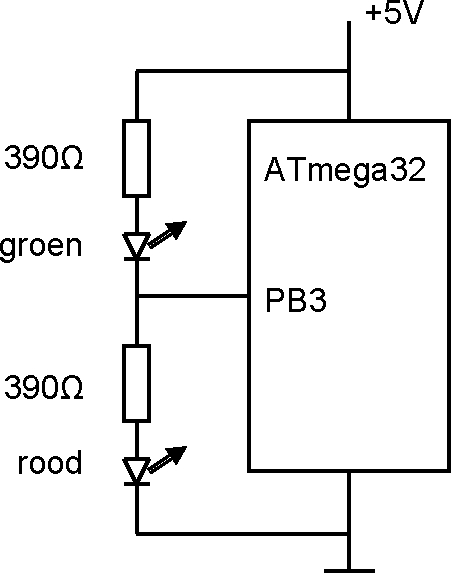
\includegraphics[scale=0.55]{pINLMIC_led_schak.pdf}
  %\caption{Blokschema machine.}
  %\label{fig:opgave2}
\end{figure}
\begin{choices}
	\CorrectChoice \label{ans:opg9} \lstinline|sbi DDRB,3| \par \lstinline|cbi PORTB,3|
	\choice \lstinline|sbi DDRB,3| \par \lstinline|sbi PORTB,3|
	\choice \lstinline|cbi DDRB,3| \par \lstinline|cbi PORTB,3|
	\choice \lstinline|cbi DDRB,3| \par \lstinline|sbi PORTB,3|
\end{choices}


\question
\label{opg:opg10}
Een ATmega32 microcontroller is aangesloten op een 8 MHz kristal.
Als we met onderstaand programma een wachttijd van 100 milliseconde
willen realiseren op welke waarden moeten de registers delay1, delay2 en
delay3 dan worden ge\"{i}nitialiseerd?
\begin{lstlisting}
    loop: subi delay1,1
          sbci delay2,0
          sbci delay3,0
          brne loop
\end{lstlisting}
\begin{choices}
	\choice Delay1 = 0x30, Delay2 = 4B, Delay3 = 04
	\CorrectChoice \label{ans:opg10} Delay1 = 0x00, Delay2 = 71, Delay3 = 02
	\choice Delay1 = 0x{f}{f}, Delay2 = 34, Delay3 = 0B
	\choice Anders dan opgegeven in a, b of c.
\end{choices}


\question
\label{opg:opg11}
Wat is de maximale wachttijd die met het programma van de vorige opgave kan worden
gerealiseerd?
\begin{choices}
	\choice 4,1 seconden
	\choice 21,0 seconden
	\choice 6,7 seconden
	\CorrectChoice \label{ans:opg11} 10,5 seconden
\end{choices}


\question
\label{opg:opg12}
Bekijk de volgende code. Welke uitspraak is correct?
\begin{lstlisting}
    ldi r16,0b01100000
    out GICR,r16
    ldi r16,0b00001100
    out MCUCR,r16
\end{lstlisting}
\begin{choices}
	\CorrectChoice \label{ans:opg12} INT0 is geactiveerd.
	\choice INT1 reageert op beide flanken
	\choice INT0 wordt geactiveerd als flankgevoelige interrupt.
	\choice INT1 is geactiveerd en reageert op een opgaande flank
\end{choices}


\question
\label{opg:opg13}
De uitkomst van een rekenkundige bewerking kan nul opleveren, dus de uitgangen van de
ALU zijn alle 0. De Z-flag van het Status Register wordt dan 1. Dit kan geregeld worden met een
logische functie. Zie onderstaande figuur. Welke logische functie is dit (er zijn geen
geinverteerde signalen beschikbaar)?
\begin{figure}[H]
  \centering
    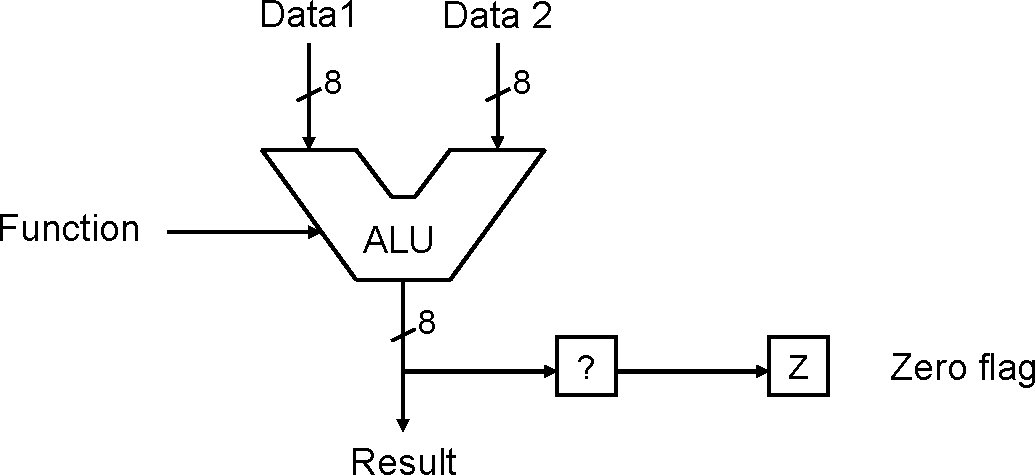
\includegraphics[scale=0.55]{pINLMIC_zero_flag.pdf}
  %\caption{Blokschema machine.}
  %\label{fig:opgave2}
\end{figure}
\begin{choices}
	\choice AND
	\choice EXOR
	\CorrectChoice \label{ans:opg13} NOR
	\choice NAND
\end{choices}


\newpage
\question
\label{opg:opg14}
Bekijk de volgende code
\begin{lstlisting}
    ldi r16,0b00011011
    out TCCR0,r16
\end{lstlisting}
\begin{choices}
	\choice T/C0 staat in de normal mode met prescaler op 1024
	\CorrectChoice \label{ans:opg14} T/C0 staat in de CTC-mode met prescaler 64 en OC0 op Toggle On Compare Match
	\choice T/C0 staat in de normal mode met prescaler 256 en OC0 op Set On Compare Match
	\choice T/C0 staat anders ingesteld dan aangegeven in a, b of c.
\end{choices}


\question
\label{opg:opg15}
Een ATmega32 wordt geklokt op 7,3728 MHz. T/C0 moet elke 16,67 ms een OCM-interrupt
genereren. De waarde voor de prescaler en OCR0 zijn dan:
\begin{choices}
	\choice prescaler = 256, OCR0 = 480
	\CorrectChoice \label{ans:opg15} prescaler = 1024, OCR0 = 119
	\choice prescaler = 64, OCR0 = 100
	\choice prescaler = 1024, OCR0 = 255
\end{choices}


\question
\label{opg:opg16}
Een ATmega32 loopt op 3,579545 MHz. Wat bedraagt de tijd tussen twee overflowinterrupts
van T/C0 als prescalerwaarde 256 wordt gebruikt?
\begin{choices}
	\CorrectChoice \label{ans:opg16} 18,3 ms
	\choice 10,1 ms
	\choice 54,6 ms
	\choice 23,5 ms
\end{choices}


\question
\label{opg:opg17}
Hieronder is het blokschema van een eenvoudige processor te vinden. De registers werken op
hetzelfde kloksignaal. De inhouden van A en B zijn onbekend. Op de ingang 'data' wordt
continu het getal 5 aangeboden. De gebruiker stuurt zelf de besturingssignalen aan (muxa...).
\begin{figure}[H]
  \centering
    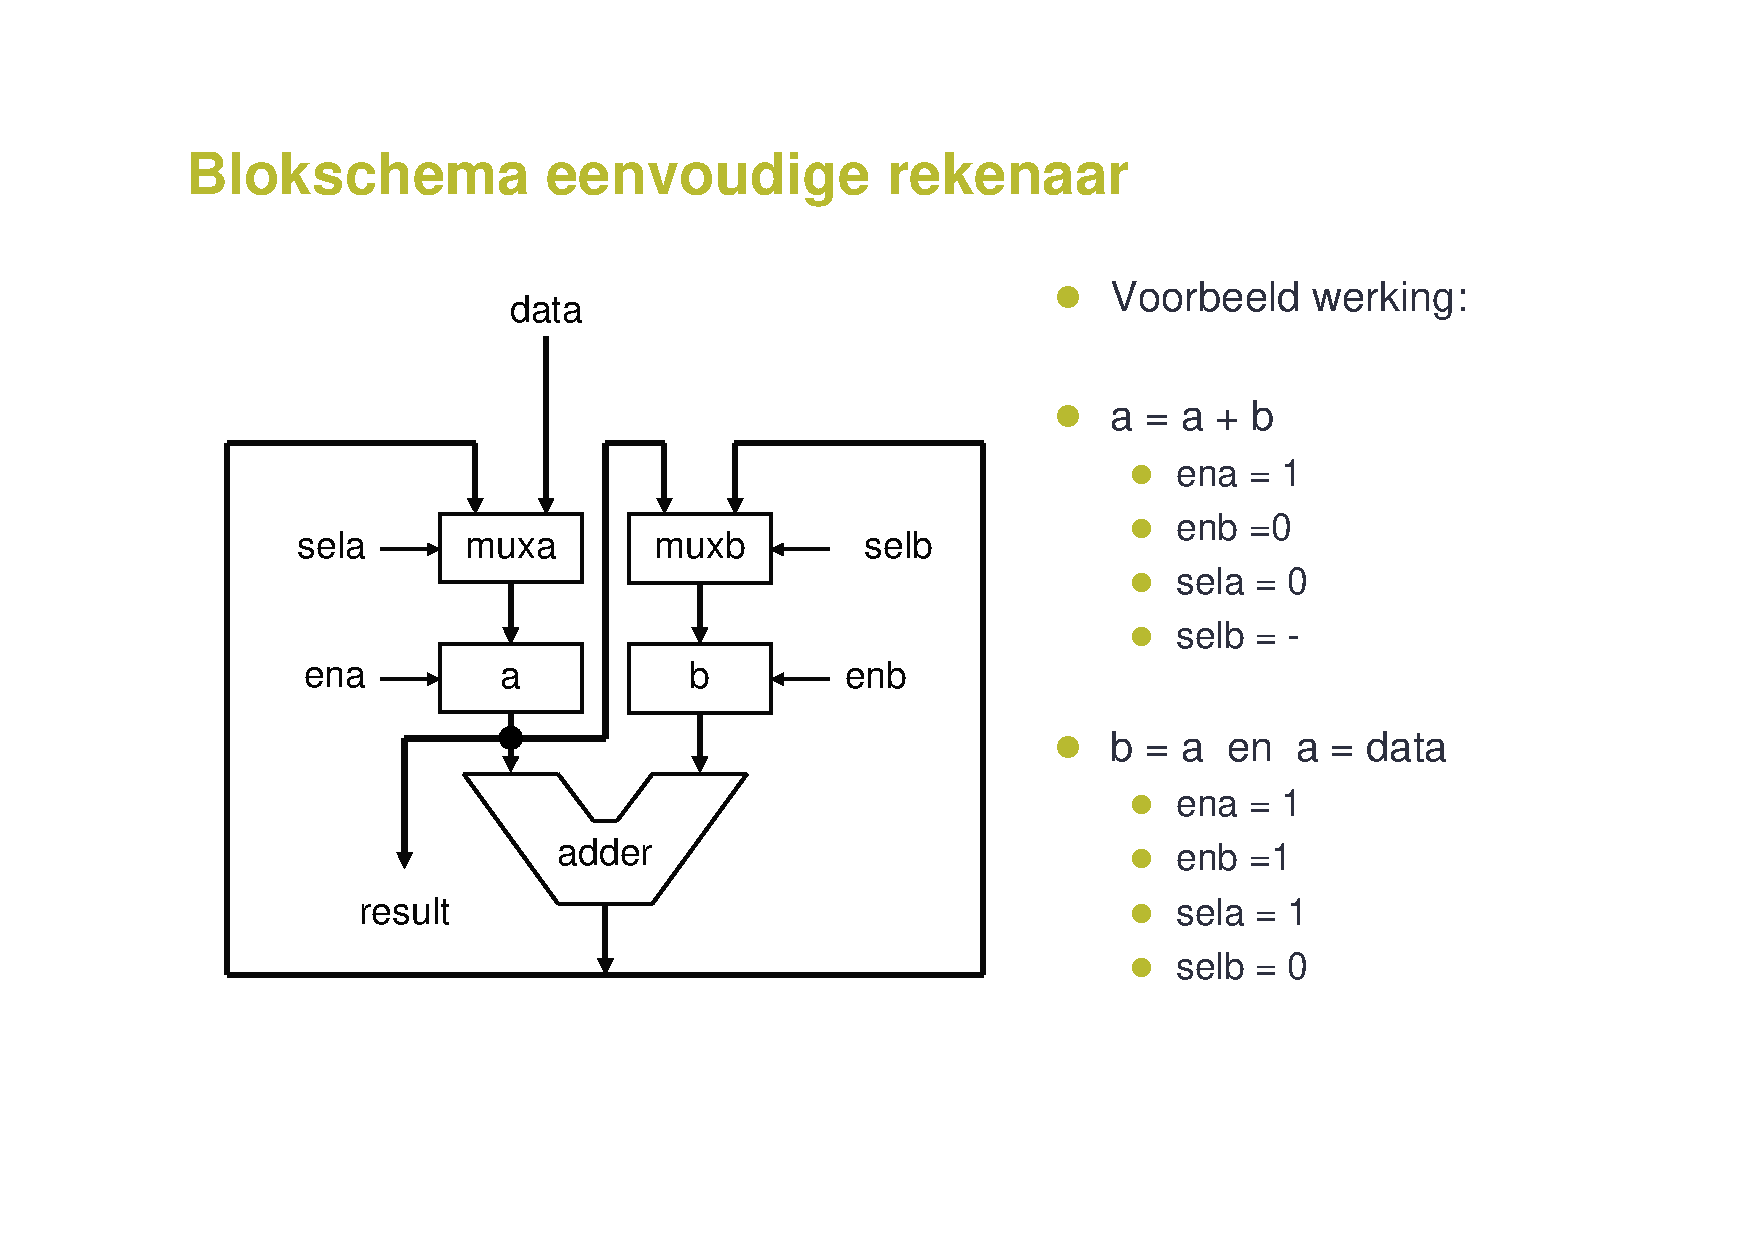
\includegraphics[scale=0.55]{pINLMIC_eenvoudige_rekenaar.pdf}
  %\caption{Blokschema machine.}
  %\label{fig:opgave2}
\end{figure}
Ontwerp nu een 'programma' dat met een minimum aan 'instructies' (aansturen van de
besturingssignalen) de waarde 35 in register B plaatst. Elke instructie kost \'{e}\'{e}n
klokpuls. Dit kost dan minimaal:
\begin{choices}
	\choice 4 klokpulsen
	\choice 5 klokpulsen
	\CorrectChoice \label{ans:opg17} 6 klokpulsen
	\choice 7 klokpulsen
\end{choices}


\question
\label{opg:opg18}
De ATmega32 microcontroller heeft 21 mogelijke interrupts. Als twee interrupts gelijktijdig
optreden, hoe verloopt dan de afhandeling van de interrupts?
\begin{choices}
	\choice Een interne interrupt wordt als eerste afgehandeld.
	\choice Een externe interrupt wordt als eerste afgehandeld.
	\choice De interrupt met het hoogste adres in de vectortabel wordt als eerste afgehandeld.
	\CorrectChoice \label{ans:opg18} De interrupt met het laagste adres in de vectortabel wordt als eerste afgehandeld.
\end{choices}


\question
\label{opg:opg19}
Gegeven de volgende code:
\begin{lstlisting}
    ; include not needed since AVR Studio 6
    ;.include "m32def.inc"
    .org 0x000
            ldi  r16,low(RAMEND)
            out  SPL,r16
            ldi  r16,high(RAMEND)
            out  SPH,r16
            ldi  r19,0xff
            ldi  r18,13
            call multi
    halt:   rjmp halt

    multi:  push r19
            push r18
            lsl  r18
            lsl  r18
            pop  r19
            add  r18,r19
            lsl  r18
            pop  r19
            ret
\end{lstlisting}

Er worden drie uitspraken gedaan:
\begin{enumerate}[itemsep=-1pt,leftmargin=23pt,label=\Roman*.]
\item De instructie \texttt{lsl} schuift de inhoud van een register naar rechts.
\item Na het uitvoeren van \texttt{multi} is R18 vermenigvuldigd met 10.
\item R19 heeft na het uitvoeren van de eerste \texttt{pop}-instructie de waarde 0x{f}{f}.
\end{enumerate}
Welke van de onderstaande uitspraken is correct?
\begin{choices}
	\CorrectChoice \label{ans:opg19} I is niet waar en II is waar
	\choice II is waar en III is waar
	\choice I is waar en II en III zijn niet waar
	\choice I is niet waar en III is waar
\end{choices}


\question
\label{opg:opg20}
Welke van de volgende uitspraken is juist/onjuist?
\begin{enumerate}[itemsep=-1pt,leftmargin=23pt,label=\Roman*.]
	\item De vlaggen kunnen geladen worden in R16.
	\item DDRC kan in R16 worden geladen d.m.v. een \texttt{lds}-instructie.
\end{enumerate}
\begin{choices}
	\choice Zowel I als II zijn onjuist
	\choice I is onjuist en II is juist
	\choice I is juist en II is onjuist
	\CorrectChoice \label{ans:opg20} Zowel I als II zijn juist.
\end{choices}


%%%\question
%%%\label{opg:opg21}
%%%Gegeven het onderstaande stukje C-code
%%%\begin{lstlisting}[language=C]
%%%\begin{verbatim}
%%%unsigned int a;
%%%unsigned int b;
%%%
%%%a = b;
%%%\end{verbatim}
%%%\end{lstlisting}
%%%Welk(e) van de onderstaande assemblercode heeft/hebben identieke werking?
%%%
%%%%\begin{lstlisting}[language=AVR]
%%%\begin{verbatim}
%%%lds r16,0x0060
%%%lds r17,0x0061
%%%sts r16,0x0062
%%%sts r17,0x0063
%%%\end{verbatim}
%%%\end{lstlisting}
%%%

\question
\label{opg:opg21}
Voor een register kan een symbolische naam gedefinieerd worden. We kunnen
register R20 bijvoorbeeld de symbolische naam ``tentamen'' geven. Wat is de
correcte wijze waarop dit in een assemblerprogramma opgegeven kan worden?
\begin{choices}
\choice \texttt{.tentamen =R20}
\choice \texttt{.db R20 =tentamen}
\CorrectChoice \label{ans:opg21} \texttt{.def tentamen =R20}
\choice \texttt{.equ tentamen =R20}
\end{choices}


\question
\label{opg:opg22}
\label{opg:rettrick}
Bij het aanroepen van een subroutine wordt het terugkeeradres op de stack opgeslagen. Dit
terugkeeradres bestaat bij de ATmega32 uit twee bytes. Het lage byte van het terugkeeradres
wordt eerst op de stack gezet, het hoge byte als tweede. Een gebruiker heeft onderstaand
programma geschreven.
\begin{lstlisting}
    ; include not needed since AVR Studio 6
    ;.include "m32def.inc"
    .org 0x000
              ldi r16,low(RAMEND)
              out SPL,r16
              ldi r16,high(RAMEND)
              out SPH,r16
              call rettrick
    loop:     rjmp loop
    
    rettrick: pop r16
              pop r16
              ldi r16,0x01
              push r16
              ldi r16,0x05
              push r16
              ret

    .org 0x0105
    halt1: rjmp halt1
    
    .org 0x0501
    halt2: rjmp halt2
\end{lstlisting}
Na uitvoeren van de \texttt{ret}-instructie wordt gesprongen naar de instructie direct achter het label
\begin{choices}
	\choice loop
	\choice rettrick
	\choice halt1
	\CorrectChoice \label{ans:opg22} halt2
\end{choices}
Hint: teken de stack tijdens uitvoering van de \texttt{CALL}-instructie en de routine \texttt{rettrick}.


\question
\label{opg:opg23}
Bestudeer het programma uit vraag \ref{opg:rettrick} aandachtig. Het Flash-ROM adres waar routine
rettrick begint is (in words):
\begin{choices}
	\choice 0x006
	\CorrectChoice \label{ans:opg23} 0x007
	\choice 0x008
	\choice 0x009
\end{choices}
Hint: slides geven aanwijzingen over de grootte van instructies.


\question
\label{opg:opg24}
Bestudeer het programma uit vraag \ref{opg:rettrick} aandachtig. De
stackpointer wordt ge\"{i}nitialiseerd 0x085f. Wat is het laagste adres dat de
stackpointer aanwijst tijdens het draaien van deze code?
\begin{choices}
	\CorrectChoice \label{ans:opg24} 0x085d
	\choice 0x085c
	\choice 0x0860
	\choice 0x085f
\end{choices}


\vskip5cm

\begin{center}
*-*-*-*-*-*-*     einde toets     *-*-*-*-*-*-*     
\end{center}


%%%%%%%%%%%%%%%%%%%%%%%%%%%%%%%%%%%%%%%%%%
%%% Answers to the questions           %%%
%%%%%%%%%%%%%%%%%%%%%%%%%%%%%%%%%%%%%%%%%%

\ifprintanswers
\newpage
\textbf{Uitwerking opgaven}
\vspace{1cm}

Opgave \ref{opg:opg1}.\label{sol:opg1}
R18 heeft de binaire waarde 0011 0110. Dit moet ge-OR-d worden met 0xA4,
binair is dat 1010 0100.

\begin{table}[h!]
	\begin{tabular}{l l l l l}
		 & \texttt{0011 0110}      &  &  0x36  &  54   \\ 
	 	 & \texttt{1010 0100 or}   &  &  0xA4  &  164  \\ 
		 & \texttt{{-}{-}{-}{-}{-}{-}{-}{-}{-}{-}{-}{-}}  &  &        &       \\ 
		 & \texttt{1011 0110}      &  &  0xB6  &  182  \\
	\end{tabular} 
\end{table}
\unskip

Het resultaat is 182 (decimaal) of 0xB6 (hexadecimaal). Het antwoord
is~\ref{ans:opg1}. Zie boek blz 177, slides week 3, pag 41.

\vspace{1em}
Opgave \ref{opg:opg2}.\label{sol:opg2}
Hier wordt een combinatie van zetten en wissen van bits
gevraagd. We noteren eerst wat er moet gebeuren: een 1 is zetten, een 0 is
wissen en een - betekent ongewijzigd laten. Een OR levert 1-en een AND levert
0-en.

\begin{table}[h!]
	\begin{tabular}{l l l l}
		 & \texttt{7654 3210}  &  &  bitnummers   \\ 
	 	 & \texttt{11{-}- 00{-}-}  &  &  wat moet er gebeuren \\ 
		 & \texttt{1100 0000}  &  &  OR-masker (1 is zetten, 0 is ongemoeid laten)    \\ 
		 & \texttt{1111 0011}  &  &  AND-masker  (0 is wissen, 1 is ongemoeid laten)  \\
	\end{tabular} 
\end{table}

Het resultaat is dus AND = 0xF3 en OR = 0xC0. Het antwoord is~\ref{ans:opg2}.
Zie boek blz 176 -- 177, slides week 3 pag 40 -- 43.
 
\vspace{1em}
Opgave \ref{opg:opg3}.\label{sol:opg3}
Op de pinnen van PORTD wordt de waarde 0x34 gezet. Dit is binair 0011 0100.
In onderstaande code wordt dit patroon eerst ingelezen in R20. Daarna wordt
er twee keer linksom geschoven. Zie onderstaande code en commentaar.

\begin{table}[h!]
	\begin{tabular}{l l l l}
		 & \texttt{in  r20,PIND}   &  &  R20 = 0011 0100  \\ 
	 	 & \texttt{lsl r20}        &  &  R20 = 0110 1000  \\ 
		 & \texttt{lsl r20}        &  &  R20 = 1101 0000  \\ 
		 & \texttt{out PORTB,r20}  &  &   \\
	\end{tabular} 
\end{table}

Het resultaat is 0xD0. Het antwoord is~\ref{ans:opg3}. Zie boek blz 186,
blz 64 -- 67, slides week 3 pag 5.

\vspace{1em}
Opgave \ref{opg:opg4}.\label{sol:opg4}
Bij  de instructie \texttt{eor ra,rb} worden de bits van register a en
register b bitsgewijs ge-exor-d. Hieronder is de bekende tabel gegeven
($n$ staat voor bitnummer 0 t/m 7).

\begin{table}[h!]
	\begin{tabular}{c c | c}
		\hline
		 $ra_{n}$ & $rb_{n}$ &  $F_{n}$  \\ \hline
		    0     &    0     &    0      \\ 
		    0     &    1     &    1      \\
		    1     &    0     &    1      \\
		    1     &    1     &    0      \\ \hline
	\end{tabular} 
\end{table}
			
Nu wordt gevraagd wat de het resultaat is van de instructie \texttt{eor r1,r1}.
Hierin wordt R1 ge-exor-d met zichzelf! Dus als bit 0 van R1 een 0 is wordt dit
bit ge-exor-d met 0. En dat levert als resultaat een 0. Precies hetzelfde
resultaat wordt verkregen als het bit een 1 is. Met andere woorden: alle bits
worden 0! Alleen de eerste en laatste regel van de tabel zijn van toepassing.
Dit is een bekende truc om een register op 0 te krijgen als een processor geen
\texttt{clr}-instructie (clear) heeft. Het antwoord is~\ref{ans:opg4}. Zie
boek blz 177 -- 178, en blz 708 (\texttt{clr}-instructie).

\vspace{1em}
Opgave \ref{opg:opg5}.\label{sol:opg5}
Willen we poortpinnen als uitgang gebruiken dan moet het DDR-register worden
geprogrammeerd met enen op de bitposities van de pinnen die als uitgang moeten
dienen. Aangezien de pinnen 0, 1, 6 en 7 als uitgang moeten worden
geprogrammeerd wordt het bitpatroon 1100.0011 en dit is gelijk aan 0xC3.
I/O-registers programmeer je met een \texttt{out}-instructie, maar dat kan
alleen vanuit een general purpose register, niet direct met een constante, dus
je hebt (bijvoorbeeld) een \texttt{ldi}-instructie nodig om een register met
een constante te laden. Zie boek blz 142~--~144, slides week 3 pag 28 -- 29.

Het anwoord is~\ref{ans:opg5}.

\vspace{1em}
Opgave \ref{opg:opg6}.\label{sol:opg6}
De \texttt{add}-instructie telt twee registers bij elkaar op waarbij de
vlaggen worden aangepast en het resultaat wordt opgeslagen.

\begin{table}[h!]
	\begin{tabular}{l l l l}
		 & \texttt{ldi r16,0x4f}   &  &  R16 = 0x4f  \\ 
	 	 & \texttt{ldi r17,0x3f}   &  &  R17 = 0x3f  \\ 
		 & \texttt{add r16,r17}    &  &  R16 = 0x4f + 0x3f = 0x8e ($>$ 0x7f dus overflow!) \\ 
	\end{tabular} 
\end{table}

Nu is 0x4f + 0x3d = 0x8e $>$ 0x7f, dus past niet in een 2's complement 8-bit
register, daarom wordt de V-flag op 1 gezet. Het msb is 1 dus de N-flag wordt
ook op 1 gezet. Beschouw je de inhouden van de registers als unsigned, dat past
het resultaat wel, dus de C-flag is 0. De Z-flag is natuurlijk 0. Zie boek
blz boek blz 162, blz 170 -- 175, blz 72 -- 73, slides week 3 pag~18.

Het antwoord is~\ref{ans:opg6}.

\vspace{1em}
Opgave \ref{opg:opg7}.\label{sol:opg7}
De microcontroller heeft geen \texttt{adc}-instructie maar die
kunnen we wel nabootsen (bij multibyte optellingen $>$ 2 bytes wordt het
lastig!). De truc is om eerst de minst significante bytes op te tellen,
daaruit volgt een carry (die kan 0 of 1 zijn). Als de carry 1 is, moet er
bij de meest significante bytes \'{e}\'{e}n worden opgeteld (dat is immers de
werking van de carry). Dus als de carry 1 is verhogen we de meest significante
bytes met \'{e}\'{e}n en anders niet. Dit is een werkje voor de
\texttt{brcc}-instructie. Als laatste moeten de twee meest significante bytes
worden opgeteld. De eventuele carry die daaruit volgt, verwaarlozen we. Als je
de code bekijkt, zie je dat er twee register-``paren'' zijn: R21 met R20 en R25
met R24.

Code I voldoet. Als eerste wordt een \texttt{add}-instructie uitgevoerd die R20
en R24 bij elkaar optelt. Als de carry 0 is, wordt over de
\texttt{subi}-instructie gesprongen. Is de carry 1, dan ``springt'' de
\texttt{brcc}-instructie niet en wordt de \texttt{subi}-instructie uitgevoerd,
die 1 bij R21 optelt. Daarna wordt in beide gevallen R25 bij R21 opgeteld.

Code II werkt niet correct. Immers de tweede \texttt{add}-instructie verknoeit
de waarden van de vlaggen die uit de eerste \texttt{add}-instructie zijn
voortgekomen, dus ook de carry-flag.

Zie boek blz 163, slides week 2 pag 15. Het antwoord is~\ref{ans:opg7}.

\vspace{1em}
Opgave \ref{opg:opg8}.\label{sol:opg8}
Zie slides week 3, pagina 36, derde item. DDR eerst naar 0, dan PORT naar 1.
De \texttt{cbi}- en \texttt{sbi}-instructies worden uitgelegd in het boek
blz 149 -- 152, zie ook boek blz 142~--~144, slides wk3 pag 39.
Het antwoord is~\ref{ans:opg8}.

\vspace{1em}
Opgave \ref{opg:opg9}.\label{sol:opg9}
Dit is een grappige schakeling waarbij je twee leds kan aansturen als ze niet
tegelijkertijd moeten branden. Aangezien een poortpin van de ATmega32 zowel
20 mA kan leveren als opnemen, geeft dit geen problemen. Om de groene
led te laten branden moet PB3 natuurlijk als een harde 0 geprogrammeerd zijn,
dus DDRB3 = 1 en PORTB3 = 0. Zie boek blz 142~--~144, blz 149 -- 152, slides
week 3 pag 29.

Nog veel leuker is dat PB3 ook gebruikt kan worden in de Output Compare Match
modus, die je kan laten toggelen. Daarmee kan je de beide leds (ogenschijnlijk)
op halve intensiteit laten branden. In de PWM-modi kan je nog veel leukere
dingen doen. Zie slides week 5, pag~30~--~34.

Het antwoord is~\ref{ans:opg9}.

\vspace{1em}
Opgave \ref{opg:opg10}.\label{sol:opg10}
Hiervoor moet je de formule gebruiken voor het bepalen van het
aantal keer dat de lus doorlopen moet worden, zie slides week 4, pag 9.
\begin{equation*}
aantal\_lussen = \dfrac{f_{cpu} \cdot wachttijd}{klolpulsen/lus}=
                 \dfrac{8000000 \cdot 0,1}{5} = 160000
\end{equation*} 

Het getal dat gebruik moet worden is 160000 en dat is 0x027100. Dan wordt
\texttt{delay1} = 0x00, \texttt{delay2} = 0x71 en \texttt{delay3} = 0x02.

Het antwoord is~\ref{ans:opg10}.

Noot: de manier waarop wachtlussen in het boek worden uitgelegd is niet
handig, dat kost veel rekenwerk. Daarnaast levert het veel instructies op
en is lastig te tunen.

\vspace{1em}
Opgave \ref{opg:opg11}.\label{sol:opg11}
Om een wachtlus maximaal tijd te laten verstoken, moet je het lus-aantal
maximaal zien te krijgen. Daarvoor moeten \texttt{delay1}, \texttt{delay2} en
\texttt{delay3} geladen worden met 0x00, hoger kan niet. Dit kan omdat er eerst
verlaagd wordt en dan pas getest op 0. Het aantal keer dat de lus dan doorlopen
wordt is 16777216 keer. Nu verbouwen we de de formule uit de slides van week 4.
\begin{equation*}
aantal\_lussen = \dfrac{f_{cpu} \cdot wachttijd}{klolpulsen/lus} 
                 \Longleftrightarrow wachttijd = 
                 \dfrac{aantal\_lussen \cdot klolpulsen/lus}{f_{cpu}}
\end{equation*} 
\begin{equation*}
wachttijd = \dfrac{16777216 \cdot 5}{8000000} = 10,485... 
            \approx 10,5 \: \text{s}
\end{equation*} 

Het antwoord is~\ref{ans:opg11}. Zie slides week 4, pag 9.

\vspace{1em}
Opgave \ref{opg:opg12}.\label{sol:opg12}
Zoek eerst de registers en de betekenissen op in het boek blz 376 -- 380
of de slides week 5, pagina 16 -- 20. Hieronder de code met commentaar.

\begin{table}[h!]
	\begin{tabular}{l l l l}
		 & \texttt{ldi r16,0b01100000}   &  &  INT0 en INT2 actief  \\ 
	 	 & \texttt{out GICR,r16}         &  &    \\ 
		 & \texttt{ldi r16,0b00001100}   &  &  INT1 op flank, INT0 op level \\ 
	 	 & \texttt{out MCUCR,r16}        &  &    \\ 
	\end{tabular} 
\end{table}

A is correct want INT0 wordt geactiveerd. B is niet correct want INT1 is
ingesteld op opgaande flank (en reageert helemaal niet, wat het staat uit).
C is niet correct want INT0 is geactiveerd als niveau-interrupt. D is niet
correct want INT1 is niet geactiveerd. Het antwoord is~\ref{ans:opg12}.

\vspace{1em}
Opgave \ref{opg:opg13}.\label{sol:opg13}
De Z-flag kan eenvoudig worden bepaald door alle uitkomstbits in \'{e}\'{e}n
NOR-poort te stoppen. De formule is dus:
\begin{equation*}
Z = \oline{R7+R6+R5+R4+R3+R2+R1+R0}
\end{equation*} 
Je kan het ook anders defini\"{e}ren: Z wordt 1 als alle uitkomstbits 0 zijn.
Dat is in formulevorm:
\begin{equation*}
Z = \oline{R7}\cdot\oline{R6}\cdot\oline{R5}\cdot\oline{R4}\cdot
    \oline{R3}\cdot\oline{R2}\cdot\oline{R1}\cdot\oline{R0}
\end{equation*}
Maar hiervoor heb je de ge\"{i}nverteerde uitgangen nodig. Met behulp van De
Morgan kan je hieruit naar de bovenste formule omwerken. Zie boek blz 71,
slides week 3, pag 18.

Het antwoord is~\ref{ans:opg13}.

\vspace{1em}
Opgave \ref{opg:opg14}.\label{sol:opg14}
Bekijk de volgende code

\begin{table}[h!]
	\begin{tabular}{l l l l}
		 & \texttt{ldi r16,0b00011011}   &  &  T/C0 in CTC mode, prescaler op 64  \\ 
	 	 & \texttt{out TCCR0,r16}        &  &  maar ook OCM-mode op Toggle on Compare Match  \\ 
	\end{tabular} 
\end{table}

Zie boek blz 315, slides week 5 pag 31 -- 34. Het antwoord is~\ref{ans:opg14}.

\vspace{1em}
Opgave \ref{opg:opg15}.\label{sol:opg15}
Deze vraag kan worden opgelost met de formule uit de slides week 5, pag 40.
Hiervoor moet de frequentie van het OCM-interrupt signaal worden uitgerekend,
want het staat als tijd genoteerd. Een periodetijd van 16,67 ms is gelijk aan
een frequentie van 60 Hz (frequentie van het lichtnet in Amerika). De
prescaler moet op 1024, de andere mogelijkheden leveren geen goede waarden
voor N en OCR0.
\begin{equation*}
prescaler \cdot N = \dfrac{f_{clk}}{f_{ocm}} 
              \longrightarrow N = \dfrac{f_{clk}}{f_{ocm} \cdot prescaler}
			= \dfrac{7372800}{60 \cdot 1024} = 120
\end{equation*} 

Let erop dat OCR0 119 moet zijn, want de timer telt van 0 t/m 119. Het
antwoord is~\ref{ans:opg15}. Zie ook boek blz 328 -- 330, blz 374 -- 375.

\vspace{1em}
Opgave \ref{opg:opg16}.\label{sol:opg16}
Ook hier wordt een tijd gevraagd, terwijl de formule van frequentie uitgaat.
De frequentie van het kristal is erg nauwkeurig gegeven en je kan deze ook
echt kopen!
\begin{equation*}
f_{o} = \dfrac{\dfrac{f_{clk}}{prescaler}}{256} = 
        \dfrac{f_{clk}}{prescaler \cdot 256} = 54,6
\end{equation*}

De frequentie is 54,6 Hz, dus de periodetijd is 18,3 ms. Het antwoord
is~\ref{ans:opg16}. Zie boek blz 369, slides week 5 pag 38.

\vspace{1em}
Opgave \ref{opg:opg17}.\label{sol:opg17}
Hieronder is wederom het blokschema van een eenvoudige processor te vinden.
De registers werken op hetzelfde kloksignaal. De inhouden van A en B zijn
onbekend. Op de ingang \texttt{data} wordt continue het getal 5 aangeboden. Er
zijn twee klokpulsen (``slagen'') nodig om beide registers met 5 geladen te
hebben, immers alleen A kan data van buitenaf ontvangen. Daarna is het een
kwestie van smaak. Hieronder zie je een mogelijkheid, er zijn ook andere. Je
moet goed opletten dat jouw mogelijk ook echt kan. Het is bijvoorbeeld niet
mogelijk om de inhoud van register B in register A te laden, omdat daar geen
hardwarevoorziening voor is. Na de $6^{\text{e}}$ klokpuls heeft register B de
waarde~35.

\begin{figure}[H]
  \begin{minipage}[!t]{0.60\linewidth}
    \centering
	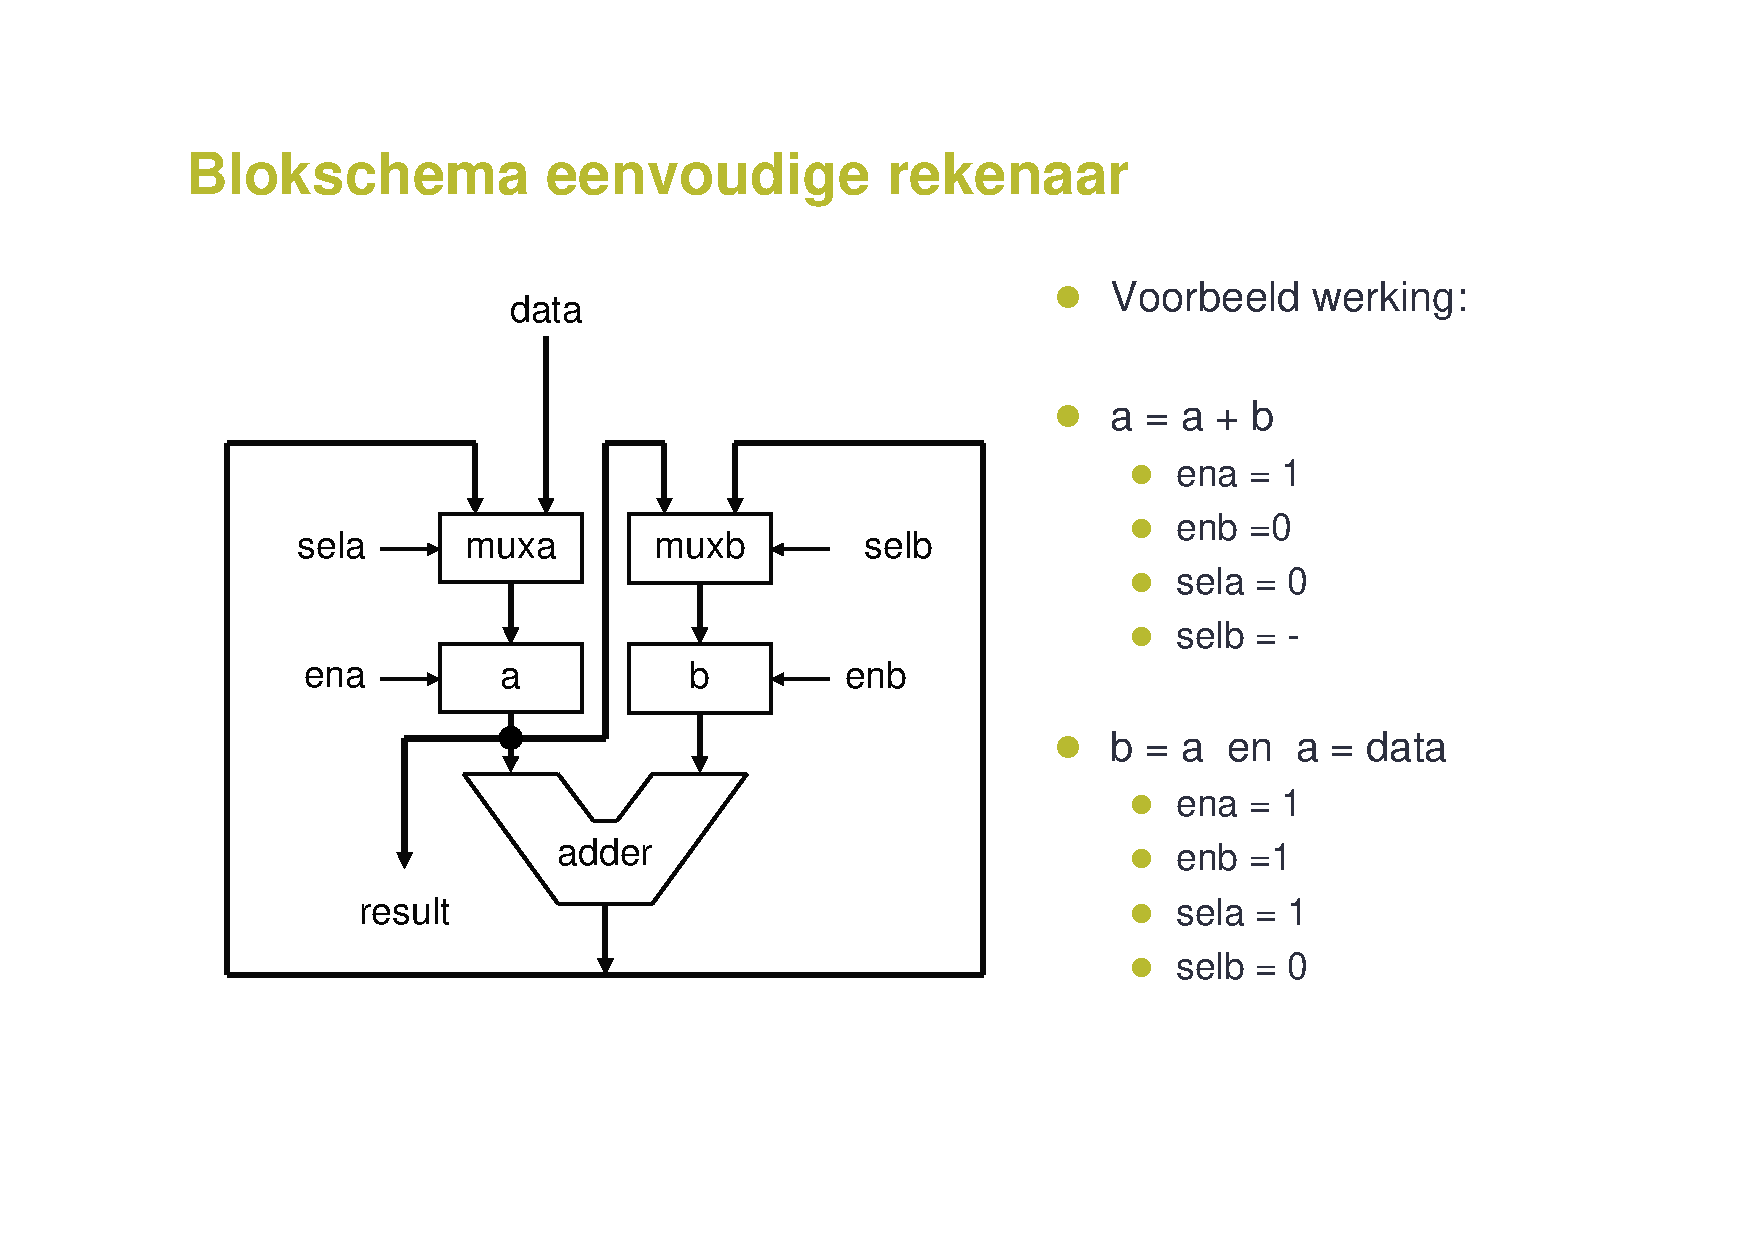
\includegraphics[scale=0.55]{pINLMIC_eenvoudige_rekenaar.pdf}
  \end{minipage}\hfill
  \begin{minipage}[!t]{.350\linewidth}
  	% Tell Latex it's a table
    \begin{tabular}{ c | c c }
      \hline
                &       &               \\ [-2.9ex]
       Klokpuls &  A    &  B     \\ \hline
           0    &  ?    &  ?     \\
           1    &  5    &  ?     \\
           2    &  5    &  5     \\
           3    &  5    &  10    \\
           4    &  15*  &  15*   \\
           5    &  5**  &  30    \\
           6    &  5    &  35    \\ \hline
    \end{tabular}
    
    * A en B tegelijk laden.
    
    ** A wordt weer geladen met 5.
    
    Er zijn andere mogelijkheden.
    \vskip10pt
  \end{minipage}\hfill
\end{figure}

Het antwoord is~\ref{ans:opg17}. Zie slides week 1, pag 37 -- 38.

\vspace{1em}
Opgave \ref{opg:opg18}.\label{sol:opg18}
Als tegelijk twee of meerdere interrupts worden aangevraagd, wordt degene met
het laagste adres in de vectortabel als eerste uitgevoerd. Zie boek blz 381,
blz 365, slides week~5, pag 13. 

Het antwoord is~\ref{ans:opg18}.

\vspace{1em}
Opgave \ref{opg:opg19}.\label{sol:opg19}
We bekijken alleen subroutine \texttt{multi}, de rest in niet
van belang. Hieronder nog de code. Achter de code ook gelijk commentaar.
\begin{lstlisting}
1   multi:  push r19       ; R19 later nodig
2           push r18       ; R18 even saven, later weer nodig
3           lsl  r18       ; Hierna is R18 = R18*2
4           lsl	 r18       ; Hierna is R18 = R18*2*2 (= R18*4)
5           pop	 r19       ; R19 laden met oude waarde R18 (let op pushes!)
6           add	 r18,r19   ; Hierna is R18 = R18*2*2 + R18 (= R18*5)
7           lsl	 r18       ; Hierna is R18 = (R18*2*2 + R18)*2 (= R18*10)
8           pop	 r19       ; Nu nog even R19 ophalen (eerste push)
9           ret            ; En terugkeren
\end{lstlisting}

Zoals je ziet vermenigvuldigt deze routine R18 met 10. De truc is om gebruik
te maken van een combinatie van schuiven (vermenigvuldigen met 2) en optellen.
Eerst wordt R19 gepushd (regel 1) op stack omdat we R19 nodig hebben voor de
optelling (regel 5 en 6). Dan wordt R18 nog eens gepushd (regel 2) omdat later
die waarde nodig is voor de optelling via R19 (regels 5 en 6). Nu wordt R18
twee keer geschoven wat een vermenigvuldiging met 4 betekent (regels 3 en 4).
Dan moet er \'{e}\'{e}n keer de originele waarde van R18 bij worden opgeteld
om een vermenigvuldiging met 5 te krijgen. R18 is natuurlijk allang veranderd
dus we moeten een tweede register gebruiken. Dit is R19. R19 popt nu de stack
(en daar werd als laatste de originele waarde van R18 opgezet! Zie slides week
4 pag 25) en telt dit op bij R18 (regels 5 en 7). Dan wordt er nog \'{e}\'{e}n
keer geschoven en heb je als resultaat dat R18 vermenigvuldigd is met 10!

Bij de code van opgave 19 worden weer drie uitspraken gegeven:

I. De instructie \texttt{lsl} schuift de inhoud van een register naar rechts.\\ 
II. Na het uitvoeren van \texttt{multi} is R18 vermenigvuldigd met 10.\\
III. R19 heeft na het uitvoeren van de eerste \texttt{pop}-instructie de
waarde 0x{f}{f}.

I is niet waar: \texttt{lsl} schuift de inhoud naar links. Zie boek, blz 186.

II is waar: zie het verhaal hierboven.

III is niet waar: laatste \texttt{push} was die van R18 en de eerste
\texttt{pop} is die van R19, m.a.w.\@ de (originele) waarde van R18 komt in
R19 (zie slides week 4, pag 24).

Het antwoord is~\ref{ans:opg19}.

\vspace{1em}
Opgave \ref{opg:opg20}.\label{sol:opg20}
Er worden twee uitspraken gedaan:

I is juist: je kan met \texttt{in r16,SREG} de vlaggen laden in register 16.
Zie boek blz 64, blz 194, blz 384, slides week 5, pag 10.

II is ook juist: DDRC is dan wel een I/O-register maar die zijn gemapd in het
DATA-bereik vanaf adres 0x0020. Je moet dat wel het nieuwe adres even
uitrekenen, en het is niet effici\"{e}nt: de \texttt{lds}-instructie is twee
words en de \texttt{in}-instructie is \'{e}\'{e}n word. Zie boek blz 59 -- 62,
blz 66, slides week 2, pag 31. 

Het antwoord is~\ref{ans:opg20}.

\vspace{1em}
Opgave \ref{opg:opg21}.\label{sol:opg21}

Zie slides week 2, pag 48. Het antwoord is~\ref{ans:opg21}. Noot: in het boek
wordt geen gebruik gemaakt van \texttt{.def}, in alle voorbeelden worden de
namen van de registers gebruikt.

\vspace{1em}
Opgave \ref{opg:opg22}.\label{sol:opg22}
Hier zie je mooi een truc om het terugkeeradres aan te passen. De truc is om
in de subroutine twee keer een \texttt{pop} te doen. Hierdoor wordt het
gestackte terugkeeradres ''van de stack'' gehaald (in feite wordt alleen de
stack pointer verhoogd). Dan pushen we zelf twee waarden op de stack en voeren
vervolgens een \texttt{ret}-instructie uit!

\begin{lstlisting}
rettrick: pop r16        ; pop stack, high byte RET-address
          pop r16        ; pop stack, low byte RET-address
          ldi r16,0x01   ; put 0x01 on stack as low byte for RET
          push r16 
          ldi r16,0x05   ; put 0x05 on stack as high byte for RET
          push r16 
          ret            ; And let's return!!!!!
\end{lstlisting}

\newpage
Hieronder de stack tijdens uitvoering:

Stack direct n\'{a} uitvoering \texttt{call}: \hspace{20pt} Stack vlak
v\'{o}\'{o}r de uitvoering van \texttt{ret}:

\begin{lstlisting}
    +------+                      +------+
    |  ..  |    <- sp             |  ..  | <-- sp           0x85d
    +------+                      +------+
    | 0x00 |                      | 0x05 |                  0x85e
    +------+                      +------+
    | 0x05 |                      | 0x01 |                  0x85f
    +------+                      +------+
\end{lstlisting}

Het terugkeeradres is dus 0x0501. Het antwoord is~\ref{ans:opg22}.
Zie ook boek blz 118 -- 127, slides week~4, pag 24.

\vspace{1em}
Opgave \ref{opg:opg23}.\label{sol:opg23}
Deze lijkt wat lastig, maar je komt een heel eind als je bedenkt dat de meeste
instructies slechts \'{e}\'{e}n word beslaan. Alleen \texttt{lds},
\texttt{sts}, \texttt{call} en \texttt{jmp}-instructies beslaan twee words.

Het programma begint op adres 0x000 (zie de \texttt{.org}-directive),
\texttt{ldi} en \texttt{out} kosten ieder \'{e}\'{e}n word. De \texttt{call}
kost twee words en de \texttt{rjmp} (relative jump) kost \'{e}\'{e}n word.
Alles tezamen is dit 8 words en het adres subroutine \texttt{rettrick} is dus
0x007 want het eerste word ligt op adres 0x000. Vergelijk het met array's in
C. Een array van 4 items loopt van 0 t/m 3.

Je kan \'{e}\'{e}n en ander opzoeken in het boek blz 118 (\texttt{call}), blz
87, 91 (\texttt{ldi}), blz 93 (\texttt{out}), blz~117 (\texttt{rjmp}) en
de slides week 3, pag 2 -- 15.

Het antwoord is~\ref{ans:opg23}.

\vspace{1em}
Opgave \ref{opg:opg24}.\label{sol:opg24}
Zie het plaatje van de stack bij het antwoord van vraag \ref{opg:opg22}.
Het laagste adres is 0x085d.

Het antwoord is~\ref{ans:opg24}.


\bigskip\bigskip
De antwoorden op een rij:
\medskip

\begin{tabular}{p{5cm} p{5cm} p{5cm}}
  \ref{opg:opg1} \ref{ans:opg1} & \ref{opg:opg9} \ref{ans:opg9}   & \ref{opg:opg17} \ref{ans:opg17} \\ 
  \ref{opg:opg2} \ref{ans:opg2} & \ref{opg:opg10} \ref{ans:opg10} & \ref{opg:opg18} \ref{ans:opg18} \\ 
  \ref{opg:opg3} \ref{ans:opg3} & \ref{opg:opg11} \ref{ans:opg11} & \ref{opg:opg19} \ref{ans:opg19} \\ 
  \ref{opg:opg4} \ref{ans:opg4} & \ref{opg:opg12} \ref{ans:opg12} & \ref{opg:opg20} \ref{ans:opg20} \\ 
                                &                                 &                                 \\ 
  \ref{opg:opg5} \ref{ans:opg5} & \ref{opg:opg13} \ref{ans:opg13} & \ref{opg:opg21} \ref{ans:opg21} \\ 
  \ref{opg:opg6} \ref{ans:opg6} & \ref{opg:opg14} \ref{ans:opg14} & \ref{opg:opg22} \ref{ans:opg22} \\ 
  \ref{opg:opg7} \ref{ans:opg7} & \ref{opg:opg15} \ref{ans:opg15} & \ref{opg:opg23} \ref{ans:opg23} \\ 
  \ref{opg:opg8} \ref{ans:opg8} & \ref{opg:opg16} \ref{ans:opg16} & \ref{opg:opg24} \ref{ans:opg24} \\ 
\end{tabular}   

%%%%% Write all correct answers to file
\makeatletter
\AtEndDocument{%
  \if@filesw
    %% Create a new file (pointer?)
    \newwrite\tempfile

	\immediate\openout\tempfile=answers.ans
	\immediate\write\tempfile
		{\@percentchar}
	\immediate\write\tempfile
		{\@percentchar\space Automaticly generated mastercard components}
	\immediate\write\tempfile
		{\@percentchar\space for exam \tisdexam@toetsnaam\space dd \tisdexam@toetsdatumkort}
	\immediate\write\tempfile
		{\@percentchar\space File written at \number\year/\two@digits\month/\two@digits\day} % doesn't behave well
	\immediate\write\tempfile
		{\@percentchar}
	\immediate\write\tempfile
		{}
	\immediate\write\tempfile
   		{\string\newcommand{\string\examcreatorname}{\tisdexam@opsteller}}%
	\immediate\write\tempfile
   		{\string\newcommand{\string\examstudentnumber}{00000000}}%
	\immediate\write\tempfile
   		{\string\newcommand{\string\examusername}{Mastercard}}%
	\immediate\write\tempfile
   		{\string\newcommand{\string\examcoursename}{\tisdexam@toetsnaam}}%
	\immediate\write\tempfile
   		{\string\newcommand{\string\examversion}{A}}%
	\immediate\write\tempfile
   		{\string\newcommand{\string\examdate}{\tisdexam@toetsdatumkort}}%
	\immediate\write\tempfile
   		{\string\newcommand{\string\examcomment}{Cesuur: 0 goed = 1, \nummultquestions\space goed = 10\string\newline\space Lineaire verdeling}}%
	\immediate\write\tempfile
   		{\string\newcommand{\string\examaq}{%
   			\getrefnumber{opg:opg1}\getrefnumber{ans:opg1},%
   			\getrefnumber{opg:opg2}\getrefnumber{ans:opg2},%
   			\getrefnumber{opg:opg3}\getrefnumber{ans:opg3},%
   			\getrefnumber{opg:opg4}\getrefnumber{ans:opg4},%
   			\getrefnumber{opg:opg5}\getrefnumber{ans:opg5},%
   			\getrefnumber{opg:opg6}\getrefnumber{ans:opg6},%
   			\getrefnumber{opg:opg7}\getrefnumber{ans:opg7},%
   			\getrefnumber{opg:opg8}\getrefnumber{ans:opg8},%
   			\getrefnumber{opg:opg9}\getrefnumber{ans:opg9},%
   			\getrefnumber{opg:opg10}\getrefnumber{ans:opg10},%
   			\getrefnumber{opg:opg11}\getrefnumber{ans:opg11},%
   			\getrefnumber{opg:opg12}\getrefnumber{ans:opg12},%
   			\getrefnumber{opg:opg13}\getrefnumber{ans:opg13},%
   			\getrefnumber{opg:opg14}\getrefnumber{ans:opg14},%
   			\getrefnumber{opg:opg15}\getrefnumber{ans:opg15},%
   			\getrefnumber{opg:opg16}\getrefnumber{ans:opg16},%
   			\getrefnumber{opg:opg17}\getrefnumber{ans:opg17},%
   			\getrefnumber{opg:opg18}\getrefnumber{ans:opg18},%
   			\getrefnumber{opg:opg19}\getrefnumber{ans:opg19},%
   			\getrefnumber{opg:opg20}\getrefnumber{ans:opg20},%
   			\getrefnumber{opg:opg21}\getrefnumber{ans:opg21},%
   			\getrefnumber{opg:opg22}\getrefnumber{ans:opg22},%
   			\getrefnumber{opg:opg23}\getrefnumber{ans:opg23},%
   			\getrefnumber{opg:opg24}\getrefnumber{ans:opg24}%
   		}}%
	\immediate\write\tempfile
   		{\string\newcommand{\string\examenglish}{no}}%
    \immediate\closeout\tempfile
  \fi
}% AtEndDocument
\makeatother

\fi


\end{questions}

\end{document}